\documentclass[tikz,border=5pt]{standalone}
\usepackage[T1]{fontenc}
\usepackage{lmodern,amsmath,amssymb}
\usetikzlibrary{arrows.meta,calc,positioning,fit,backgrounds,shapes.geometric,matrix,decorations.pathreplacing,patterns}
\definecolor{ink}{gray}{0.08}
\definecolor{wash}{gray}{0.965}
\definecolor{soft}{gray}{0.45}
\tikzset{box/.style={draw=ink,line width=.65pt,fill=white,align=center,inner sep=4pt,outer sep=0pt,font=\small},flow/.style={draw=ink,line width=.65pt,-{Latex[length=1.8mm,width=1.3mm]},rounded corners=2pt},annotation/.style={font=\scriptsize,text=soft,align=center},groupbox/.style={draw=soft,dashed,line width=.45pt,fill=wash}}
\begin{document}
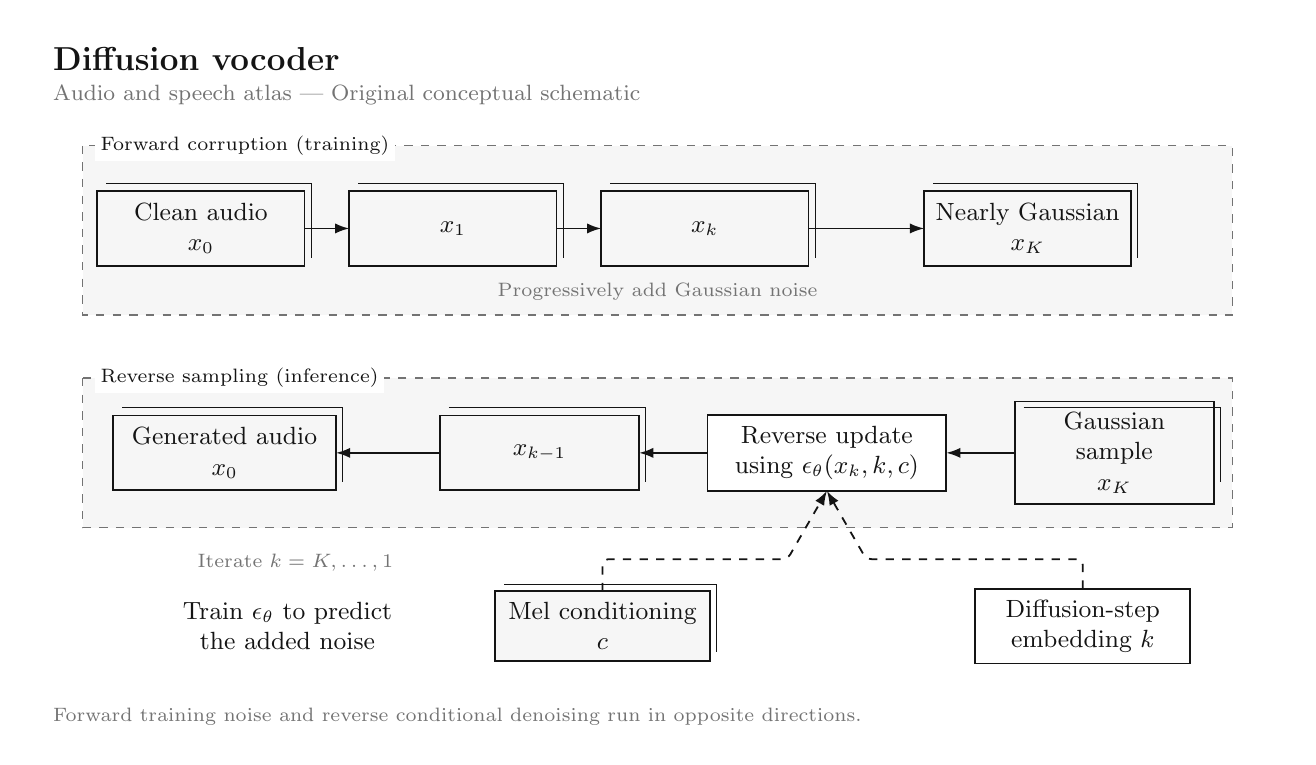
\begin{tikzpicture}[x=1cm,y=-1cm,font=\rmfamily,text=ink]

\path[use as bounding box] (0,0) rectangle (16,9);
\node[anchor=west,font=\large\bfseries] at (.2,.4) {Diffusion vocoder};
\node[anchor=west,font=\footnotesize,text=soft] at (.2,.85) {Audio and speech atlas | Original conceptual schematic};
\begin{pgfonlayer}{background}
\draw[groupbox] (0.7,1.5) rectangle (15.299999999999999,3.65);
\node[anchor=west,font=\scriptsize,fill=white,inner sep=2pt] at (0.85,1.5) {Forward corruption (training)};
\draw[groupbox] (0.7,4.45) rectangle (15.299999999999999,6.35);
\node[anchor=west,font=\scriptsize,fill=white,inner sep=2pt] at (0.85,4.45) {Reverse sampling (inference)};
\end{pgfonlayer}
\node[box,fill=wash,minimum width=2.6cm,minimum height=0.95cm,text width=2.35cm] (x0) at (2.2,2.55) {Clean audio\\$x_0$};
\draw[ink,line width=.4pt] (1.0000000000000002,1.9749999999999996) -- (3.6,1.9749999999999996) -- (3.6,2.925);
\node[box,fill=wash,minimum width=2.6cm,minimum height=0.95cm,text width=2.35cm] (x1) at (5.4,2.55) {$x_1$};
\draw[ink,line width=.4pt] (4.2,1.9749999999999996) -- (6.8,1.9749999999999996) -- (6.8,2.925);
\node[box,fill=wash,minimum width=2.6cm,minimum height=0.95cm,text width=2.35cm] (xk) at (8.6,2.55) {$x_k$};
\draw[ink,line width=.4pt] (7.3999999999999995,1.9749999999999996) -- (10.0,1.9749999999999996) -- (10.0,2.925);
\node[box,fill=wash,minimum width=2.6cm,minimum height=0.95cm,text width=2.35cm] (xK) at (12.7,2.55) {Nearly Gaussian\\$x_K$};
\draw[ink,line width=.4pt] (11.499999999999998,1.9749999999999996) -- (14.1,1.9749999999999996) -- (14.1,2.925);
\node[box,fill=wash,minimum width=2.5cm,minimum height=0.95cm,text width=2.25cm] (noise) at (13.8,5.4) {Gaussian sample\\$x_K$};
\draw[ink,line width=.4pt] (12.65,4.825000000000001) -- (15.15,4.825000000000001) -- (15.15,5.775);
\node[box,minimum width=3.0cm,minimum height=0.95cm,text width=2.75cm] (step) at (10.15,5.4) {Reverse update\\using $\epsilon_\theta(x_k,k,c)$};
\node[box,fill=wash,minimum width=2.5cm,minimum height=0.95cm,text width=2.25cm] (state) at (6.5,5.4) {$x_{k-1}$};
\draw[ink,line width=.4pt] (5.35,4.825000000000001) -- (7.85,4.825000000000001) -- (7.85,5.775);
\node[box,fill=wash,minimum width=2.8cm,minimum height=0.95cm,text width=2.55cm] (clean) at (2.5,5.4) {Generated audio\\$x_0$};
\draw[ink,line width=.4pt] (1.2000000000000002,4.825000000000001) -- (4.0,4.825000000000001) -- (4.0,5.775);
\node[box,fill=wash,minimum width=2.7cm,minimum height=0.85cm,text width=2.45cm] (condition) at (7.3,7.6) {Mel conditioning\\$c$};
\draw[ink,line width=.4pt] (6.049999999999999,7.075) -- (8.75,7.075) -- (8.75,7.925000000000001);
\node[box,minimum width=2.7cm,minimum height=0.85cm,text width=2.45cm] (time) at (13.4,7.6) {Diffusion-step\\embedding $k$};
\begin{pgfonlayer}{background}
\draw[flow] (x0.east) -- (x1.west);
\draw[flow] (x1.east) -- (xk.west);
\draw[flow] (xk.east) -- (xK.west);
\draw[flow] (noise.west) -- (step.east);
\draw[flow] (step.west) -- (state.east);
\draw[flow] (state.west) -- (clean.east);
\draw[flow,dashed] (condition.north) -- (7.3,6.75) -- (9.65,6.75) -- (step.south);
\draw[flow,dashed] (time.north) -- (13.4,6.75) -- (10.65,6.75) -- (step.south);
\end{pgfonlayer}
\node[align=center,anchor=center,font=\scriptsize,text=soft,text width=10cm] at (8,3.35) {Progressively add Gaussian noise};
\node[align=center,anchor=center,font=\scriptsize,text=soft,text width=4.8cm] at (3.4,6.8) {Iterate \mbox{$k=K,\ldots,1$}};
\node[align=center,anchor=center,font=\small,text=ink,text width=4.8cm] at (3.3,7.6) {Train \mbox{$\epsilon_\theta$} to predict\\the added noise};
\node[anchor=west,align=left,font=\scriptsize,text=soft,text width=15.6cm] at (.2,8.75) {Forward training noise and reverse conditional denoising run in opposite directions.};
\end{tikzpicture}
\end{document}
